\documentclass[a4paper, 12pt]{article}

\usepackage[T1]{fontenc}
\usepackage[utf8]{inputenc}

\usepackage{roboto}
\usepackage{parskip}
\usepackage[english]{babel}
\usepackage{a4wide}
\usepackage{graphicx}
\usepackage{svg}

\title{intelliPhoto 0.31 - Manual}
\author{Paul Norberger \& the intelliPhoto team}

\begin{document}
\begin{titlepage}
\maketitle
\thispagestyle{empty}
\begin{center}

\includegraphics[width=0.35\linewidth,keepaspectratio]{assets/icon}
\end{center}
\tableofcontents
\end{titlepage}
\section{Introduction}
intelliPhoto is a software for creating and editing graphics of various kinds. While it allows for work with a full color space, it will also allow export in a more restriced format, which uses 1 byte per pixel. Currently its in its early stages of development and has a very limited array of tools as well as a functional, but barebones interface. This will change in future versions.
Currently the following features are implemented, which will be described in further detail on the following pages:
\begin{itemize}
\item A barebones user interface
\item Loading and Saving images from and to standardized formats (such as .png, .bmp or .jpg)
\item Drawing with a pen with adjustable width and color, clearing the whole canvas with one color and drawing lines, rectangles, circles and polygons as well as flood filling adjacent pixels
\item A layer structure, that allows for creating, deleting, moving and changing the order of layers
\end{itemize}

\section{User Guide}
After startup the following window opens:
\begin{center}
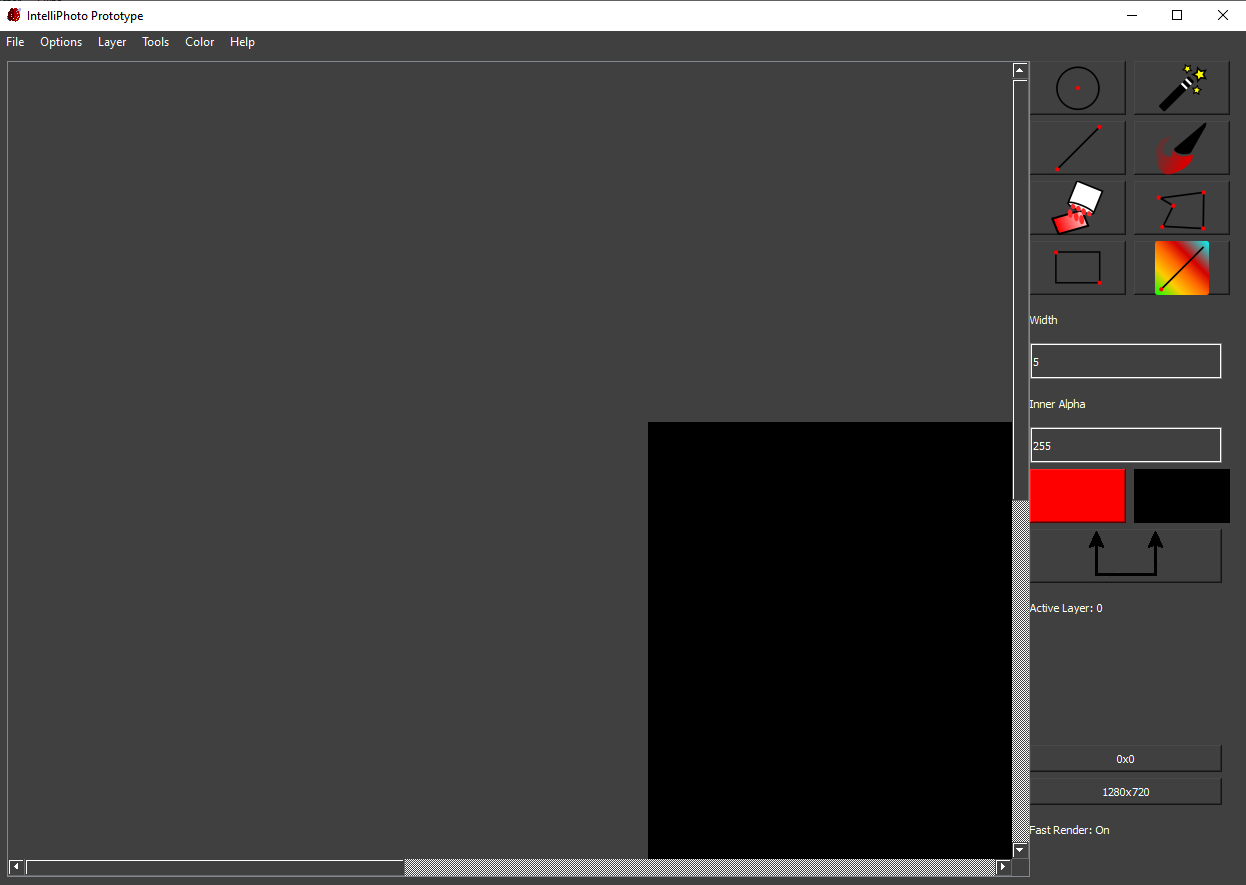
\includegraphics[width=0.55\linewidth,keepaspectratio]{assets/startup}
\end{center}

\subsection{Loading images}
To load a preexisting image, click on \texttt{File} in the top menu bar and then on \texttt{Open...} in the appearing context menu.
\begin{center}
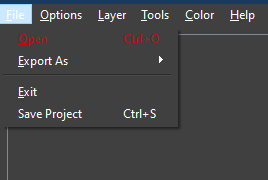
\includegraphics[width=0.3\linewidth,keepaspectratio]{assets/file-open}
\end{center}

A file explorer window opens. Navigate to the image you want to open and click on \texttt{Open} or the equivalent in your system language. The image will now be imported and displayed.

\subsection{Saving images}
To save the current canvas as an image, click on \texttt{File} in the top menu bar then hover over \texttt{Save As} and click on your preferred file format in the appearing context menu.
\begin{center}
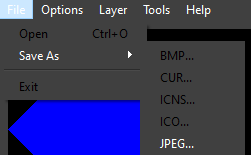
\includegraphics[width=0.3\linewidth,keepaspectratio]{assets/file-save}
\end{center}

A file explorer window opens. Navigate to your preferred save location, input a file name and click on \texttt{Save} or the equivalent in your system language. The image will be saved at that location in the selected file format.

\subsection{Setting the active layer}
The active layer is the layer you are currently editing. To change it, you currently have to specify the index of the layer under \texttt{Layer > select Active...}.

\subsection{Setting the main and secondary color}
The main and secondary color are a concept used by all the drawing tools. You select them independendly of other tool parameters under \texttt{Tools > Color}.
\begin{center}
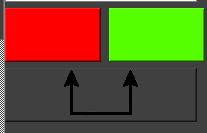
\includegraphics[width=0.3\linewidth,keepaspectratio]{assets/change-colors}
\end{center}
The appearing popup will allow you to specify a new color.

\subsection{Switching main and secondary color}
An often desired use case is to switch the main and secondary color. So that you don't have to this manually, which would be time consuming there is an easy command to do it under \texttt{Tools > Color}.
It is also bound to the keyboard shortcut \texttt{Ctrl+Shift+S}.

\subsection{Drawing with the pen tool}
To activate the pen tool simply select it under \texttt{Tools > Pen}. You will be prompted to input the pen width, just put in the width you desire.
\begin{center}

\includegraphics[width=0.2\linewidth,keepaspectratio]{assets/tool-pen}
\end{center}
To edit the active layer with the pen tool simply click and hold the left mouse button while hovering the layer on the canvas. When you click within the boundaries of the active layer, the pixels in the radius you selected will change their color to the main color which you selected under the section above.

\subsection{Drawing straight lines}
To activate the line tool select it under \texttt{Tools > Line}. You will be prompted to input the line width.
To draw a line you now have to left click on the starting point on the canvas, hold it pressed and move to the end point and release the mouse button.

You can cancel this operation at any time by clicking the right mouse button while holding the left and then releasing both.

\subsection{Fill the active layer in one color}
To fill the whole layer with the main color, you first specify the color on the right side of the picture.

\begin{center}
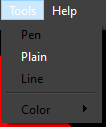
\includegraphics[width=0.3\linewidth,keepaspectratio]{assets/tool-plain}
\end{center}

\subsection{Moving layers}
The layers are flexible and can be moved to a different position on the canvas, their order can be changed at will. For this you can use the movement options under \texttt{Layer}. Keep in mind that the changes always only effect the active layer you have chosen in the section "Setting the active layer".

\begin{center}
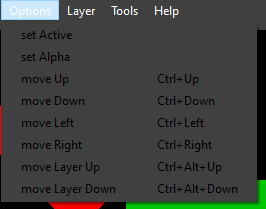
\includegraphics[width=0.3\linewidth,keepaspectratio]{assets/layer-options}
\end{center}

\subsection{Creating and deleting layers}
Raster Layers can be created at will under \texttt{Layer > New Layer...} You will be prompted to input the width and height of the new layer. Afterwards it will be created.
\begin{center}
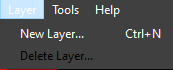
\includegraphics[width=0.3\linewidth,keepaspectratio]{assets/create-layer}
\end{center}
To delete the active layer you have to click on \texttt{Delete Layer...} in the same submenu.

\subsection{Transparency and layers}
Layers can also be made more or less transparent under \texttt{Layer > set Alpha}. Values between 0 and 255 are valid. There is currently no error handling and this can lead to memory leaks, so be careful. This also only effects the active layer.

\subsection{Closing the program}
To close the program you have to execute the exit program routine, which heavily depends on your operating system. Usually you can find a red cross symbol at the top right, though it may be different depending on your setup.
For Windows 10, the desired symbol looks like this when hovered:
\begin{center}

\includegraphics[width=0.9\linewidth,keepaspectratio]{assets/close-window}
\end{center}
Alternatively you can press \texttt{CTR+Q}.

\section{Next steps}
The following features are currently high priority and will be implimented in the near future:
\begin{itemize}
\item Refactoring the code, improving readability, structure and the dev documentation
\item Improving the UI and integrating all the tools in it
\end{itemize}

\end{document}